% Frugal AI seminar, part 5: where it runs. Hardware figures come from the manufacturer pages named in the Ref
% lines. Our own measurements are labelled with the device and the date. CheatSheet-safe: no floats.

\section[Where]{Where It Runs}

%%%%%%%%%%%%%%%%%%%%%%%%%%%%%%%%%%%%%%%%%%%%%%%%%%%
\begin{frame}[fragile]\frametitle{}
\begin{center}
{\Large Where It Runs}

\medskip
{\small (Five kinds of hardware you already have)}
\end{center}
\end{frame}

%%%%%%%%%%%%%%%%%%%%%%%%%%%%%%%%%%%%%%%%%%%%%%%%%%%
\begin{frame}[fragile]\frametitle{The Platform Map}
\begin{center}
\adjustbox{max width=\linewidth, max totalheight=0.52\textheight}{%
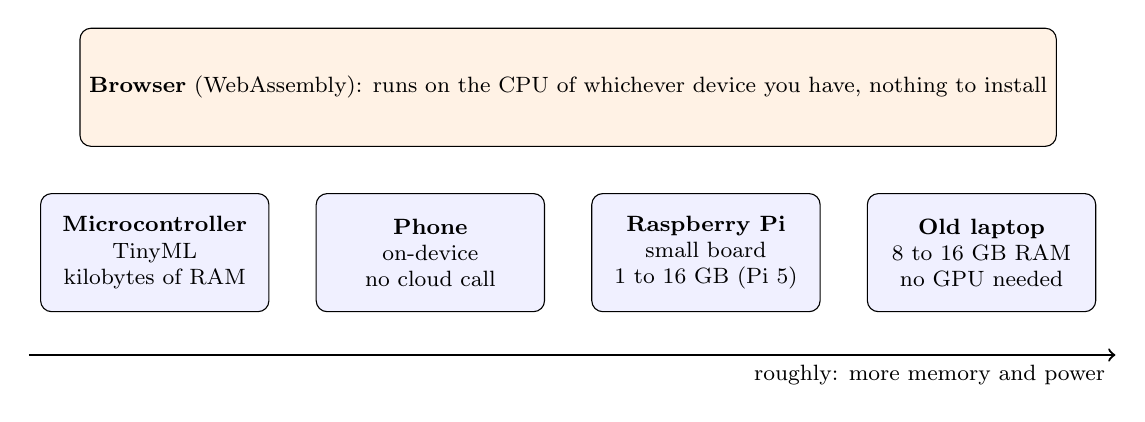
\begin{tikzpicture}
\tikzstyle{plat}=[draw, rounded corners, align=center, minimum width=2.9cm, minimum height=1.5cm, font=\footnotesize, fill=blue!6]
\node[plat] (mcu) at (0,0) {\textbf{Microcontroller}\\TinyML\\kilobytes of RAM};
\node[plat] (phone) at (3.5,0) {\textbf{Phone}\\on-device\\no cloud call};
\node[plat] (pi) at (7,0) {\textbf{Raspberry Pi}\\small board\\1 to 16 GB (Pi 5)};
\node[plat] (lap) at (10.5,0) {\textbf{Old laptop}\\8 to 16 GB RAM\\no GPU needed};
\draw[->, thick] (-1.6,-1.3) -- (12.2,-1.3) node[below left, font=\footnotesize] {roughly: more memory and power};
\node[plat, minimum width=10.4cm, fill=orange!10] (web) at (5.25,2.1) {\textbf{Browser} (WebAssembly): runs on the CPU of whichever device you have, nothing to install};
\end{tikzpicture}}
\end{center}
\begin{itemize}
\item Language models live on the right; classifiers and keyword spotters on the left.
\item The FrugalAI awesome list has one section for each platform.
\end{itemize}
\end{frame}

%%%%%%%%%%%%%%%%%%%%%%%%%%%%%%%%%%%%%%%%%%%%%%%%%%%
\begin{frame}[fragile]\frametitle{Old Laptop, CPU Only}
\begin{itemize}
\item AIOOLL (AI on an old Linux laptop) reports an Intel i3-8130U with 8 GB of RAM and an SSD, and about 8 tokens per second for Gemma2 2B.
\item The FrugalAI harness on a 10-core, 16 GB Windows PC that also has a small NVIDIA GPU (GeForce MX570, 2 GB), which LM Studio can use. Median decode speed with the GPU off (15 runs, one model loaded): Qwen3 1.7B 20.3 tokens per second, Gemma 2 2B 10.9. With the GPU on: 54.0 and 12.2. Engine memory about 2.1 GB and 3.4 GB.
\item This is a development machine, not a frugal-tier device. The small GPU helps Qwen3, which fits in its 2 GB, about 2.7 times; it barely helps Gemma, which does not fit.
\item The old Dell laptop and the Raspberry Pi: not measured yet. The method is written first (decode speed, first-token time, peak memory, a median over repeats).
\end{itemize}
{\tiny (Ref: AIOOLL README, as reported there; FrugalAI benchmarks, 19 October 2026)}
\end{frame}

%%%%%%%%%%%%%%%%%%%%%%%%%%%%%%%%%%%%%%%%%%%%%%%%%%%
\begin{frame}[fragile]\frametitle{Raspberry Pi 5}
\begin{itemize}
\item CPU: 2.4 GHz quad-core 64-bit Arm Cortex-A76. RAM: 1, 2, 4, 8 or 16 GB.
\item Power: a 5 V, 5 A USB-C supply is recommended, and the board performs best with active cooling.
\item That is enough for small language models on the CPU. The Soliga voice project (earlier) runs on Raspberry Pi hardware.
\item In FrugalAI the Pi is the next device to measure, with a power meter: nothing is claimed for it yet.
\end{itemize}
{\tiny (Ref: Raspberry Pi 5 product page)}
\end{frame}

%%%%%%%%%%%%%%%%%%%%%%%%%%%%%%%%%%%%%%%%%%%%%%%%%%%
\begin{frame}[fragile]\frametitle{Phones}
\begin{itemize}
\item On-device means no cloud call: the data stays on the phone and it works without a connection.
\item Curated lists such as awesome-mobile-llm collect mobile-first models, deployment tools, benchmarks and optimisations.
\item In FrugalAI a phone track is on the roadmap: one recipe measured on a real Android phone. Not started yet.
\item If you have run something on a phone, it belongs in the awesome list.
\end{itemize}
\end{frame}

%%%%%%%%%%%%%%%%%%%%%%%%%%%%%%%%%%%%%%%%%%%%%%%%%%%
\begin{frame}[fragile]\frametitle{Microcontrollers: TinyML}
\begin{itemize}
\item The Arduino Nano 33 BLE Sense uses a Nordic nRF52840: a 64 MHz Arm Cortex-M4F with 1 MB of flash and 256 KB of RAM.
\item It carries a microphone and a motion sensor (an IMU), among others.
\item What fits: keyword spotting, motion and vibration classification, small vision models. For a machine-monitoring job, an always-on vibration classifier is the natural example.
\item What does not: language models. Different tool for a different job.
\end{itemize}
{\tiny (Ref: Arduino Nano 33 BLE Sense documentation; Nordic nRF52840 product page)}
\end{frame}
